% LaTeX template for Lab Reports
% Copyright (C) 2014 Julian Coy

%% CHANGE REPORT TITLE HERE
\newcommand{\reporttitle}{
 FSM System Design
}

%% HEADER/PREAMBLE INFORMATION

% "The font should be 11pt Times New Roman"
\documentclass[11pt]{report}
\usepackage[T1]{fontenc}
\usepackage[utf8]{inputenc}

\usepackage{mathptmx}               

% "The body of the paper should use 1" margins on all sides."
\usepackage[margin=1in]{geometry}

% "Pages must be numbered, starting with 1 on the first page in the body of the report.
% The cover page should not be numbered. 
% Page numbers should be in the bottom-right corner of the page."
\usepackage{fancyhdr}
\pagestyle{fancy}
\fancyhead{}
\fancyfoot{}
\renewcommand{\headrulewidth}{0pt}
\fancyfoot[R]{\thepage}

% Set up customized spacing
\usepackage{setspace}

% Allows for Trademark Symbols
\usepackage{textcomp}

% Remove spacing between items in lists
\usepackage{enumitem}

% Remove extra spacing between titles of sections and subsections
\usepackage{titlesec}
\titlespacing\section{0pt}{10pt}{10pt}
\titlespacing\subsection{0pt}{10pt}{10pt}
\titlespacing\subsubsection{0pt}{0pt plus 4pt minus 2pt}{0pt plus 2pt minus 2pt}

% Setup the specialized chapter section for the Abstract
\titlespacing\chapter{0pt}{0pt plus 4pt minus 2pt}{0pt plus 2pt minus 2pt}
\titleformat{\chapter}[block]{\centering\Huge}{}{}{}{}

% Set up BibTeX integration using IEEE citation format
\usepackage{cite}
\bibliographystyle{ieeetr}
\usepackage{url}

% Set bibliography to have a section header rather than chapter header
\makeatletter
\renewenvironment{thebibliography}[1]
     {\section*{\scshape Works Cited}% <-- this line was changed from \chapter* to \section*
      \@mkboth{\MakeUppercase\bibname}{\MakeUppercase\bibname}%
      \list{\@biblabel{\@arabic\c@enumiv}}%
           {\settowidth\labelwidth{\@biblabel{#1}}%
            \leftmargin\labelwidth
            \advance\leftmargin\labelsep
            \@openbib@code
            \usecounter{enumiv}%
            \let\p@enumiv\@empty
            \renewcommand\theenumiv{\@arabic\c@enumiv}}%
      \sloppy
      \clubpenalty4000
      \@clubpenalty \clubpenalty
      \widowpenalty4000%
      \sfcode`\.\@m}
     {\def\@noitemerr
       {\@latex@warning{Empty `thebibliography' environment}}%
      \endlist}
\makeatother

% Set up math
\usepackage{amsmath}
\usepackage{amsfonts}
\usepackage{amssymb}

% Set up graphics
\usepackage{graphicx}
\usepackage{float}

% Set up tables
\usepackage{tabularx}
\usepackage{booktabs}

% Set up code blocks
% or not...

\usepackage{listings}
\usepackage{color}

\definecolor{dkgreen}{rgb}{0,0.6,0}
\definecolor{gray}{rgb}{0.5,0.5,0.5}
\definecolor{mauve}{rgb}{0.58,0,0.82}

\lstset{frame=tb,
  language=VHDL,
  aboveskip=3mm,
  belowskip=3mm,
  showstringspaces=false,
  columns=flexible,
  basicstyle={\small\ttfamily},
  numbers=none,
  numberstyle=\tiny\color{gray},
  keywordstyle=\color{blue},
  commentstyle=\color{dkgreen},
  stringstyle=\color{mauve},
  breaklines=true,
  breakatwhitespace=true
  tabsize=3
}

%% START OF DOCUMENT

\begin{document}

% "The main body of text should use 1.5 spacing"
\begin{spacing}{1.5}

% Suppress page numbering on first page
\thispagestyle{empty}

\begin{scshape}

% Title
% "The title should be centered and written in approximately 22pt font."
\vspace*{30pt}
{
\Huge
\begin{center}
    \reporttitle
\end{center}
}
\vspace{30pt}

% Team Number
% "The Team number should be centered and written several lines below the title and should use a
% similar size font as the title."
{
\Large
\begin{center}
  Lab Report 2 for ECE327 \\
  Digital Systems Design
\end{center}
}
\vspace{30pt}
% Team Members
% "Directly below the team identifier, team members should be listed alphabetically by last name, one
% per line, in approximately 14pt font. The column of names should be approximately centered on
% the page, but the names within the column should be left justified (so they all start at the same
% horizontal position)."
{
\Large 
\begin{center}
  Submitted by \\
  Julian Coy
\end{center}
}
\vspace{120pt}

{
\Large
\begin{center}
  Undergraduate of Electrical \& Computer Engineering \\
  Clemson University
\end{center}
}
\vspace{30pt}

{
\Large
\begin{center}
  March 12, 2014
\end{center}
}

\end{scshape}

% New page and reset page numbering
\clearpage

%% START EDITS BELOW %%

\vspace{15pt}
  \setcounter{chapter}{1}
  \chapter*{Abstract}
  \label{cha:abstract}
\vspace{72pt}

Finite state machines (FSMs) are the basic building blocks of complex computing.  They allow for logical implementation of algorithms, which is critical to the engineering of computing systems.  In this lab, a finite state machine is constructed to flag "stop codons" in a sample of DNA code.  The implementation of this finite machine is done though VHDL using behavioral modeling techniques.  Testbench results are provided later in this report to show a working simulation of the FSM when connected to other logical components.  The other logical components built for this lab are a Parallel-to-Serial Output (PISO) register and a counter register.  The inputs to the FSM design will be threefold.  There will be one array of 18 switches which are used to simulate the DNA input.  There will also be a "reset" button and a "load" button.  The reset button will asynchronously reset the counter block, while the load button will be used to push new data into the PISO register. This design showcases the power of finite state machine logic.  It is critical for engineers to grasp the power of logical computation and to see the scalability of such power.  By combining simple FSM logical blocks, one can create a vast and complicated algorithm with ease.

\vspace{3.5in}

\textit{Note: All clocks generated for simulation were built using Morten Zilmers clock gen package \cite{Synth}.}

\thispagestyle{empty} % clear page number
\clearpage
\setcounter{page}{1}

\section*{\scshape Introduction} %(0.5 pages)
\label{cha:introduction}

The purpose of this lab is to sequence DNA bases consisting of "T", "A", "C", and "G" and look for stop codons.  Stop codons are series of three bases that trigger the end of a DNA sequence.  The stop codons we look for in this lab are "TAA", "TGA", and "TAG".  In order to differentiate the bases, we use a binary representation for the bases (Figure \ref{fig:bases}).  The bases are then fed into the FSM, the number of stop codons are counted, and then the count is displayed on the Altera board.

\vspace{15px}
\begin{figure}[H]
    \centering
    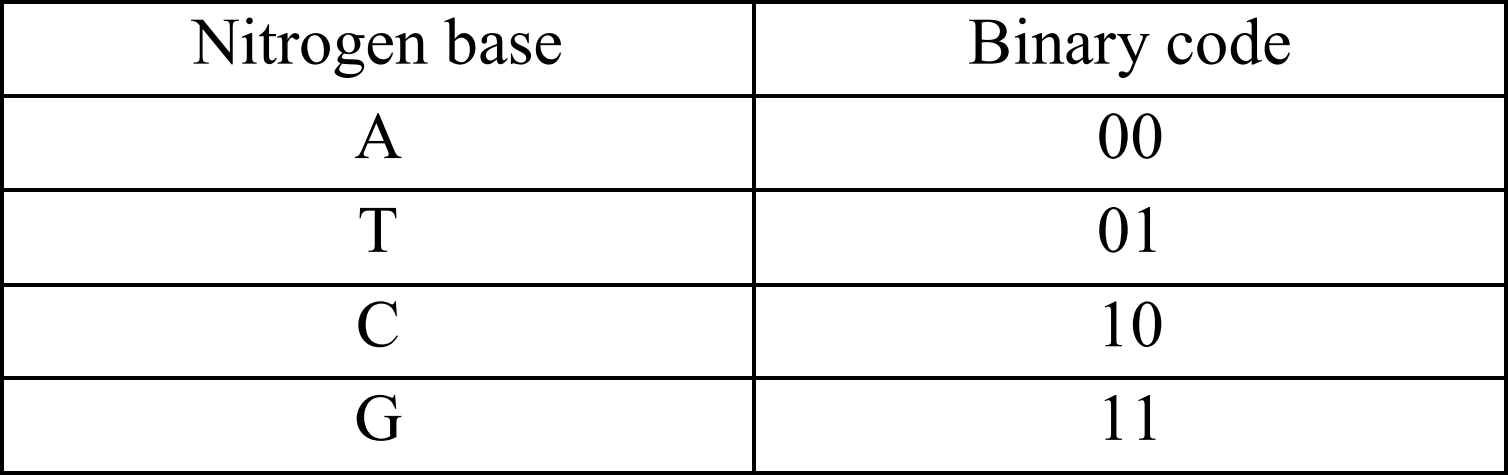
\includegraphics[width=0.6\textwidth,keepaspectratio]{bases.png}
    \caption{DNA Base Representation}
    \label{fig:bases}
\end{figure}

Lab two consists of three major logical components (the FSM logic, the counter logic, and the PISO logic) and one minor component (the LED logic).  The counter and PISO components are standalone and can be simulated through ModelSim for testing or used for implementation with other systems with minimal modifications.  The FSM logic is designed to model state transitions of the incoming DNA data from the PISO.  And the minor LED logic simply displays a number of LEDs correspondent to the output of the counter logic.

\section{\scshape FSM System Design} %(0.5 pages)
\label{sec:fsm_design}

\subsection{\scshape PISO Logic Design}
\label{sub:design_piso}

The PISO design for this lab was built specifically to handle 18 bits of input data at a time.  This was a design choice made for the layout of the Altera board, as it only allowed for 18 bits of modifiable input at a time. The PISO logic parses the 18 bits of data by 2 bit intervals.  It then outputs the first two bits of data on the rising edge of the clock.  This output is connected to the FSM input.  The PISO then shifts the data left by two bits and adds a "01" to the right end.  The "01" code was chosen for the shift packing to make sure that when the data is fully read, no extra stop codons are accidentally detected.  Since the code for the "T" base is "01" and no stop codons end with "T" or consist of all "T" bases, this eliminates that possibility.

\subsection{\scshape Testing of the PISO}
\label{sub:test_piso}

To test the PISO, a testbench was created that would send in a string of data to the PISO and monitor the output on the rising edge of the following clock cycles (Figure \ref{fig:test_piso}). Notice that the output data is not started until the rising edge of the clock cycle following the release of the load button (low active).  In the example shown, the data input is "01001100010101001" which corresponds to "TAGATTTAT".  The output is exactly what we expect. Not shown in the figure is the loading of "T" ("01") values on the preceeding end because it shows no change to the final value in the simulation.

\vspace{15px}
\begin{figure}[H]
    \centering
    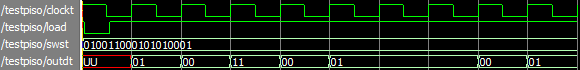
\includegraphics[width=1.0\textwidth,keepaspectratio]{piso.png}
    \caption{PISO Simulation Results}
    \label{fig:test_piso}
\end{figure}

\subsection{\scshape Counter Logic Design}
\label{sub:design_counter}

The counter is modeled behaviorally and simply counts the number of stop flags from the FSM it encounters.  The maximum count used for this project is three, but can be modified to much larger ranges with only a few lines of code.  The counter outputs its value on an integer signal that is sent to the LED logic.

\subsection{\scshape Testing of the Counter}
\label{sub:test_counter}

The counter was tested by sending stop flags to the input and periodically sending a reset signal (Figure \ref{fig:test_counter}).  The counter performed without issue even when using large integer values.  The maximum count size tested was 255, but since the maximum number of stop codons possible from the board were three, the counter integer limit was set to 3.

\vspace{15px}
\begin{figure}[H]
    \centering
    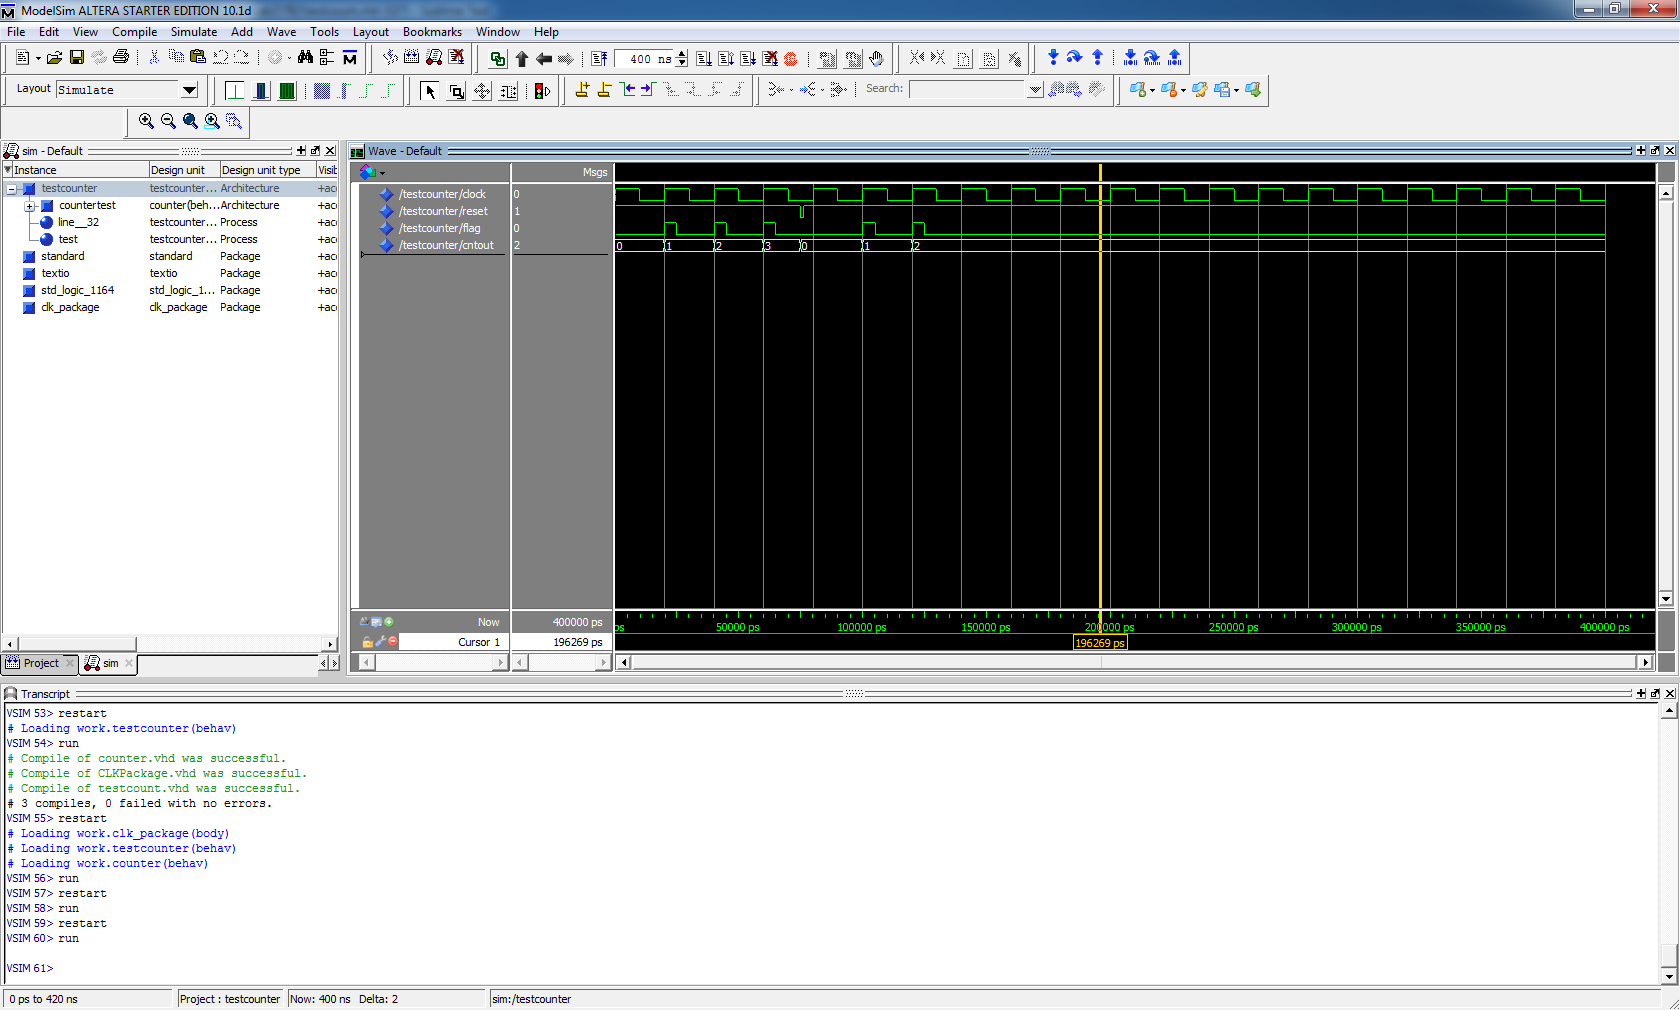
\includegraphics[width=1.0\textwidth,height=4cm,keepaspectratio]{counter.png}
    \caption{Counter Simulation Results\cite{Synth}}
    \label{fig:test_counter}
\end{figure}

\subsection{\scshape FSM Logic Design}
\label{sub:design_counter}

The FSM was designed with 4 logical states: A, B, C, and D.  The first state, A, was the reset state.  This state represents no stop codons and no detection of the beginning of any codons (which always start with a "T" base).  Once a "T" is detected the state will shift to B.  From B there are four options which are shown in Figure \ref{fig:diag_fsm}.  In the figure, the input to the FSM "w" determines the next state.  This FSM uses a Mealy design principle.  This allows for faster outputs and less state management.  In fact, to implement this in a Moore model, at least 5 states would need to be used.

\vspace{15px}
\begin{figure}[H]
    \centering
    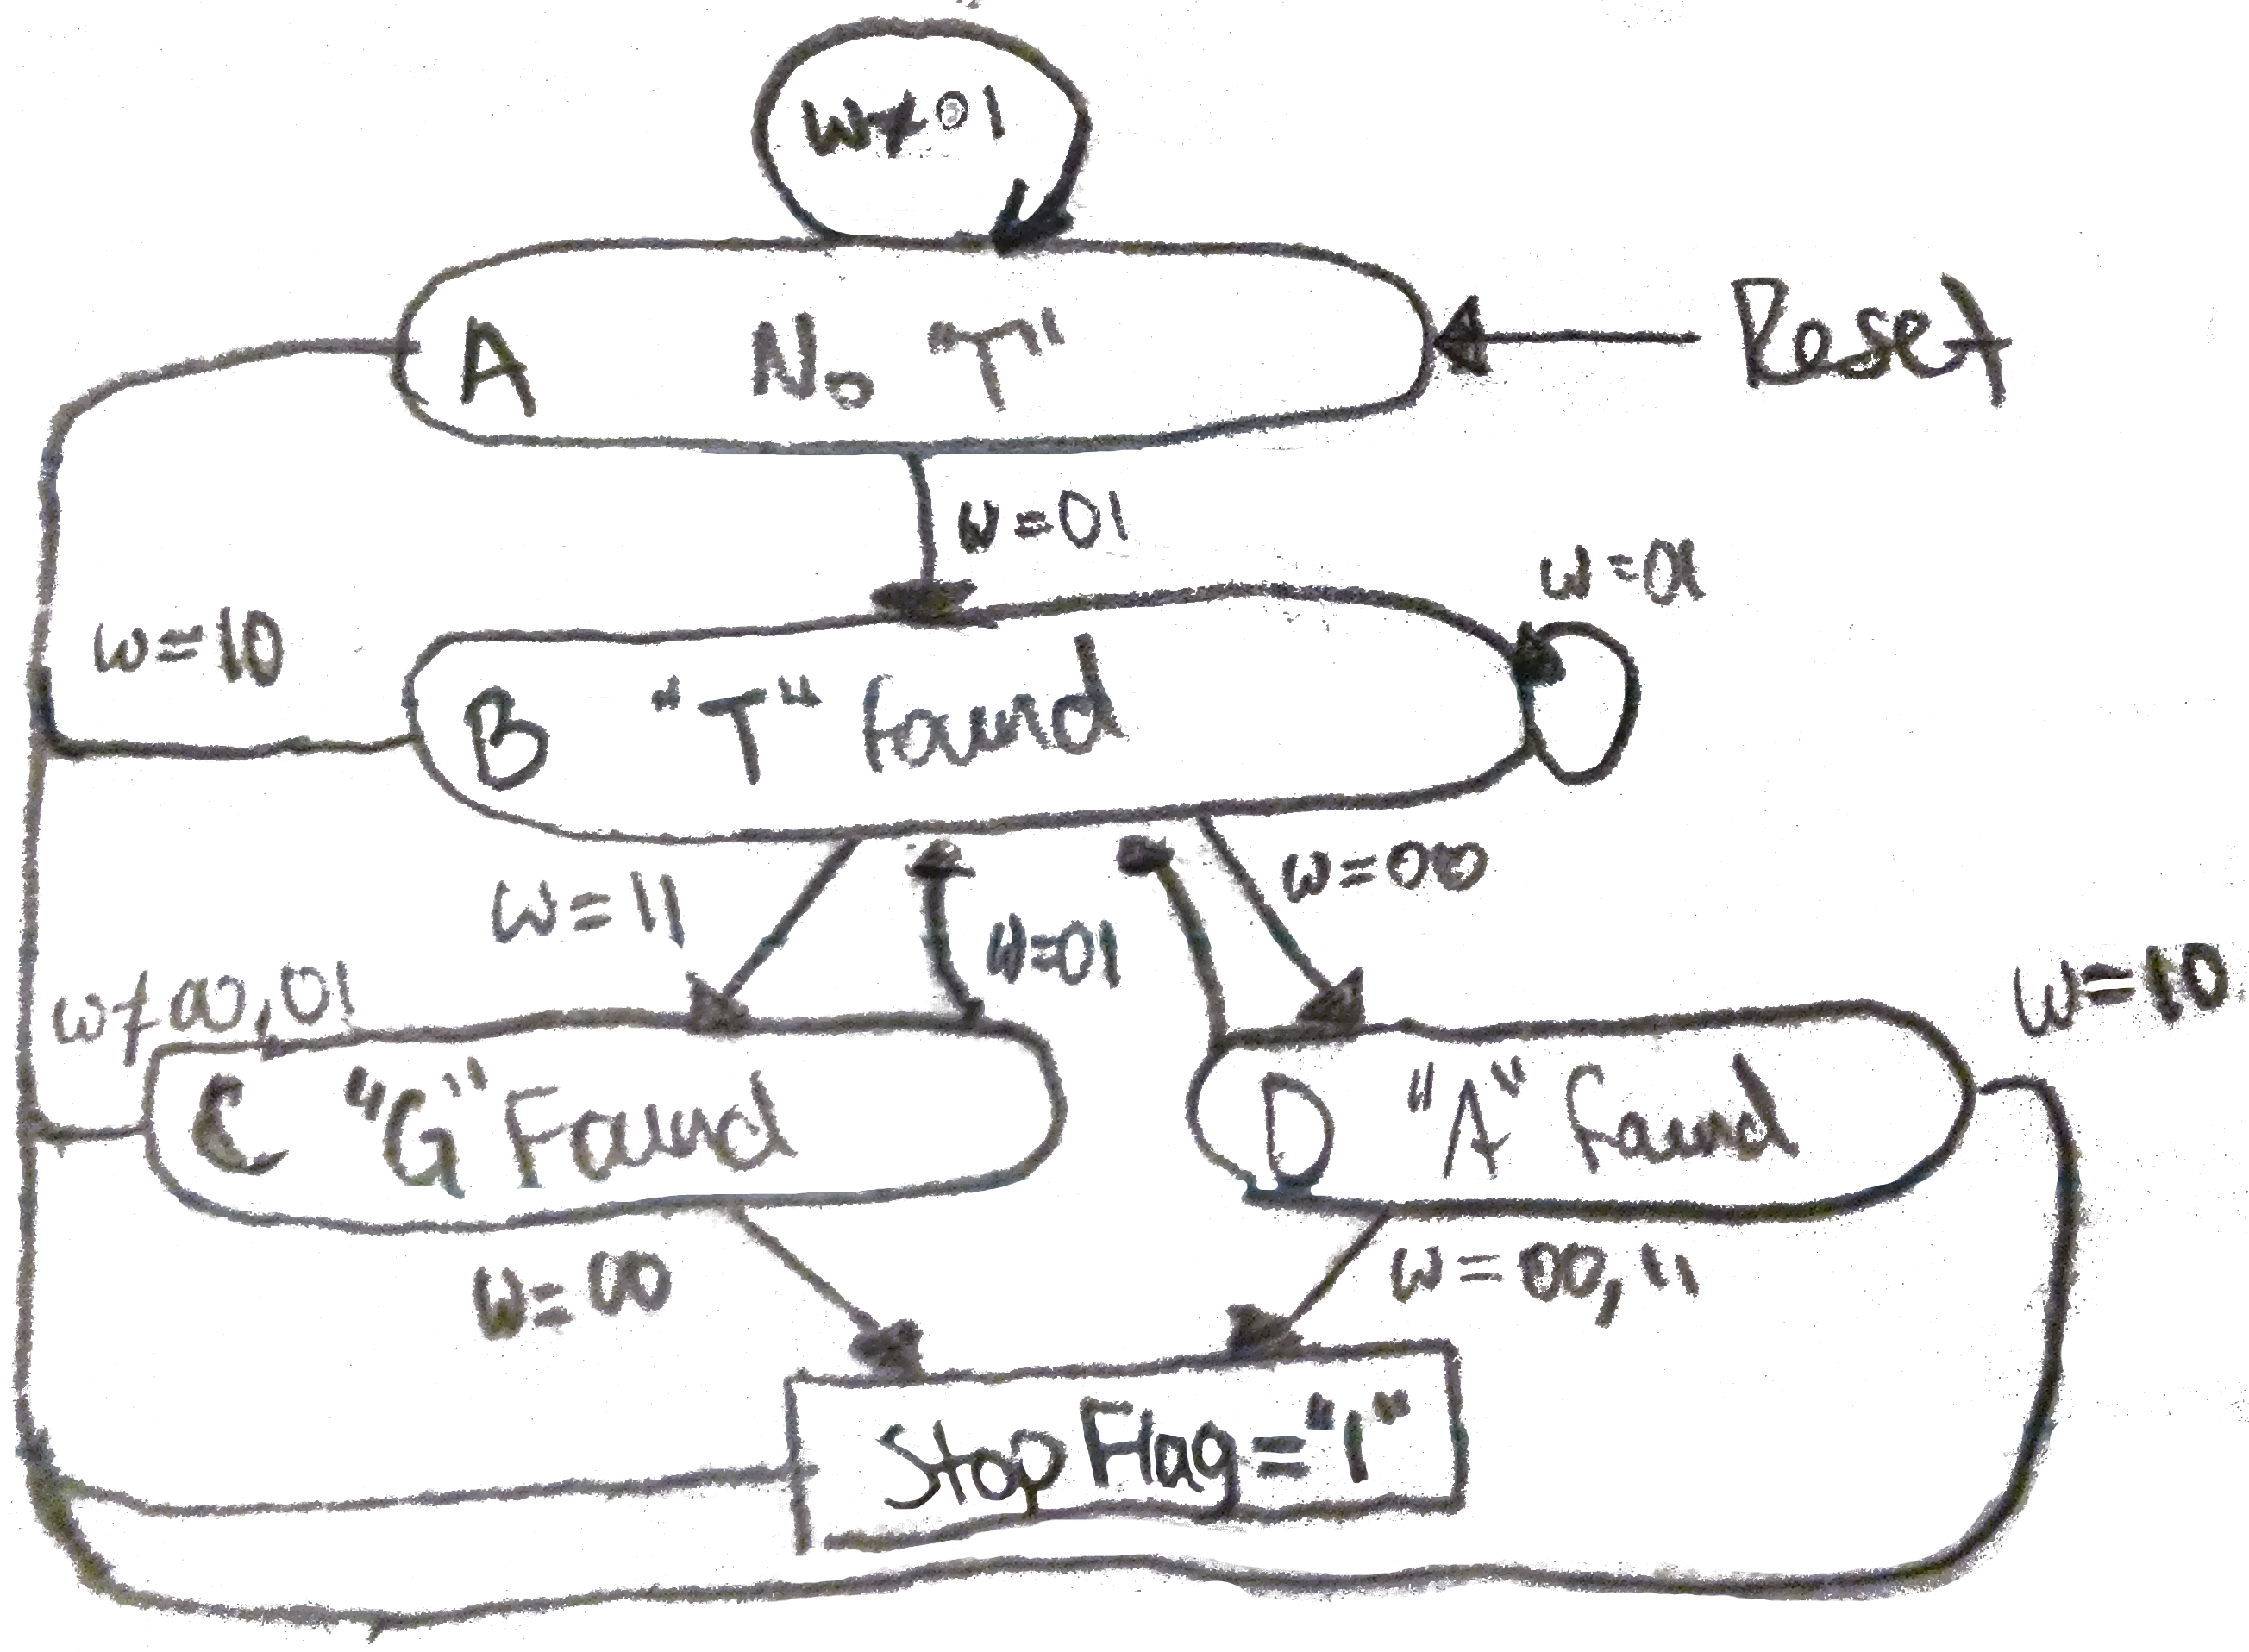
\includegraphics[width=0.7\textwidth,keepaspectratio]{fsm.png}
    \caption{FSM State Diagram}
    \label{fig:diag_fsm}
\end{figure}

Once the FSM is in state C or D it looks for specific input signals.  If the signals match a certain condition set (w=00 for C or w=00,11 for D) then the stop flag is triggered and the state resets to A.  The only danger to this model is when the asynchronous reset is called between the C and D input conditional and the stop flag assignment.  If this were to occur the counter could be prematurely incremented on the next cycle.  However, this is incredibly rare as for this to occur requires that the reset must toggle within the fraction of between a comparison and signal assignment.

\clearpage

\subsection{\scshape Testing of the FSM}
\label{sub:test_counter}

The FSM was tested by 

\vspace{15px}
\begin{figure}[H]
    \centering
    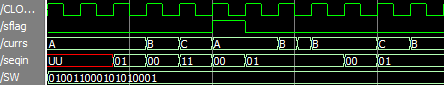
\includegraphics[width=1.0\textwidth,height=4cm,keepaspectratio]{simulation.png}
    \caption{FSM Simulation Results}
    \label{fig:test_fsm}
\end{figure}

\section{\scshape Conclusions} % (fold)
\label{sec:conclusions}

This lab is a testament to the modularity, reliability, and scope of FPGA programming with VHDL.  Simple components or systems can be designed and connected to form incredibly complex systems that can perform a wide range of actions.  Originally, the subsystems in the lab seemed unconnected to one another.  However, by the end of the lab it was clear that the systems were building upon each other.  This lab also clearly demonstrated the value of simulations in attempting to analyze complex FPGA systems.

% section scshape_conclusions (end)

% Bibliography

\clearpage

\bibliography{citationsfile}{}

\clearpage

\chapter*{\scshape Appendix A: 5-Seven Segment Decoder}
\label{app:a}

\vspace{45px}
\begin{lstlisting}
LIBRARY ieee;
USE ieee.std_logic_1164.all;
LIBRARY work;
USE work.all;

ENTITY LAB1d IS

  PORT (
    SW              : IN STD_LOGIC_VECTOR(17 DOWNTO 0);
    HEX0,HEX1,HEX2,HEX3,HEX4  : OUT STD_LOGIC_VECTOR(6 DOWNTO 0)
  );
      
END ENTITY LAB1d;

ARCHITECTURE LAB1d_arch OF LAB1d IS

  COMPONENT seven_seg_parse
    PORT (
      DATA  : IN STD_LOGIC_VECTOR(2 DOWNTO 0);
      OUTPUT  : OUT STD_LOGIC_VECTOR(6 DOWNTO 0)
    );
  END COMPONENT seven_seg_parse;

  SIGNAL S0,S1,S2,S3,S4 : STD_LOGIC_VECTOR(6 DOWNTO 0);

BEGIN
    behav : PROCESS (S0,S1,S2,S3,S4)
    BEGIN
      CASE SW(17 DOWNTO 15) IS
        WHEN "000" =>
          HEX0 <= S0;
          HEX1 <= S1;
          HEX2 <= S2;
          HEX3 <= S3;
          HEX4 <= S4;
        WHEN "001" =>
          HEX0 <= S1;
          HEX1 <= S2;
          HEX2 <= S3;
          HEX3 <= S4;
          HEX4 <= S0;
        WHEN "010" =>
          HEX0 <= S2;
          HEX1 <= S3;
          HEX2 <= S4;
          HEX3 <= S0;
          HEX4 <= S1;
        WHEN "011" =>
          HEX0 <= S3;
          HEX1 <= S4;
          HEX2 <= S0;
          HEX3 <= S1;
          HEX4 <= S2;
        WHEN "100" =>
          HEX0 <= S4;
          HEX1 <= S0;
          HEX2 <= S1;
          HEX3 <= S2;
          HEX4 <= S3;
        WHEN others =>
          HEX0 <= S0;
          HEX1 <= S1;
          HEX2 <= S2;
          HEX3 <= S3;
          HEX4 <= S4;
      END CASE;
    END PROCESS behav;
    seven_seg_0 : seven_seg_parse PORT MAP(SW(2 DOWNTO 0),S0);
    seven_seg_1 : seven_seg_parse PORT MAP(SW(5 DOWNTO 3),S1);
    seven_seg_2 : seven_seg_parse PORT MAP(SW(8 DOWNTO 6),S2);
    seven_seg_3 : seven_seg_parse PORT MAP(SW(11 DOWNTO 9),S3);
    seven_seg_4 : seven_seg_parse PORT MAP(SW(14 DOWNTO 12),S4);
END ARCHITECTURE LAB1d_arch;

-------------------------

LIBRARY ieee;
USE ieee.std_logic_1164.all;
LIBRARY work;
USE work.all;

ENTITY seven_seg_parse IS 
  
  PORT (
    DATA  : IN STD_LOGIC_VECTOR(2 DOWNTO 0);
    OUTPUT  : OUT STD_LOGIC_VECTOR(6 DOWNTO 0)
  );

END ENTITY seven_seg_parse;

ARCHITECTURE basic OF seven_seg_parse IS

BEGIN
  behav : PROCESS (DATA)
  BEGIN
    CASE DATA IS
      WHEN "000" => OUTPUT <= "0000111";
      WHEN "001" => OUTPUT <= "1111001";
      WHEN "010" => OUTPUT <= "0010000";
      WHEN "011" => OUTPUT <= "0000110";
      WHEN "100" => OUTPUT <= "1001100";
      WHEN others =>  OUTPUT <= "0000000";
    END CASE;
  END PROCESS behav;
END ARCHITECTURE basic;

LIBRARY ieee;
USE ieee.std_logic_1164.all;
LIBRARY work;
USE work.all;

ENTITY mux21 IS 

  PORT (
    SEL,X,Y : IN STD_LOGIC;
    M   : OUT STD_LOGIC);
END ENTITY mux21;

ARCHITECTURE basic OF  mux21 IS
BEGIN
  mux21_behavior : PROCESS (SEL,X,Y)
  BEGIN 
      if (SEL = '0') then M <= X; else M <= Y; END if;
  END PROCESS mux21_behavior;
END ARCHITECTURE basic;
\end{lstlisting}

\chapter*{\scshape Appendix B: Test Bench (Part 4)}
\label{app:b}

\vspace{45px}
\begin{lstlisting}
LIBRARY ieee;                                               
USE ieee.std_logic_1164.all;                                

ENTITY TB1d IS
END TB1d;

ARCHITECTURE TB1d_arch OF TB1d IS
     
  -- test signals going into and out of the mux                                                                                            
  SIGNAL TESTSO1 : STD_LOGIC_VECTOR(6 DOWNTO 0);
  SIGNAL TESTSO2 : STD_LOGIC_VECTOR(6 DOWNTO 0);
  SIGNAL TESTSO3 : STD_LOGIC_VECTOR(6 DOWNTO 0);
  SIGNAL TESTSO4 : STD_LOGIC_VECTOR(6 DOWNTO 0);
  SIGNAL TESTSO5 : STD_LOGIC_VECTOR(6 DOWNTO 0);
  SIGNAL TESTSW  : STD_LOGIC_VECTOR(17 DOWNTO 0);

  COMPONENT LAB1d
    PORT (
      SW   : IN  STD_LOGIC_VECTOR(17 DOWNTO 0);
      HEX0 : OUT STD_LOGIC_VECTOR(6 DOWNTO 0);
      HEX1 : OUT STD_LOGIC_VECTOR(6 DOWNTO 0);
      HEX2 : OUT STD_LOGIC_VECTOR(6 DOWNTO 0);
      HEX3 : OUT STD_LOGIC_VECTOR(6 DOWNTO 0);
      HEX4 : OUT STD_LOGIC_VECTOR(6 DOWNTO 0) 
    );
  END COMPONENT;

  -- map the signals

  BEGIN
  multimux : LAB1d
  PORT MAP (
    SW   => TESTSW,
    HEX0 => TESTSO1,
    HEX1 => TESTSO2,
    HEX2 => TESTSO3,
    HEX3 => TESTSO4,
    HEX4 => TESTSO5
  );

  -- start the test

  test : PROCESS                                                                                   
  BEGIN                                                         
  
  -- set the initial word to be TIGER and initial position
  TESTSW(14 DOWNTO 0)  <= "100011010001000";
  TESTSW(17 DOWNTO 15) <= "000"; WAIT FOR 4 ns;

  -- cycle around message
  TESTSW(17 DOWNTO 15) <= "001"; WAIT FOR 2 ns;
  TESTSW(17 DOWNTO 15) <= "010"; WAIT FOR 2 ns;
  TESTSW(17 DOWNTO 15) <= "011"; WAIT FOR 2 ns;
  TESTSW(17 DOWNTO 15) <= "100"; WAIT FOR 2 ns;

  -- change message
  TESTSW(17 DOWNTO 15) <= "000";
  TESTSW(14 DOWNTO 0)  <= "100001010011000"; WAIT FOR 4 ns;

  -- cycle randomly message
  TESTSW(17 DOWNTO 15) <= "011"; WAIT FOR 2 ns;
  TESTSW(17 DOWNTO 15) <= "010"; WAIT FOR 2 ns;
  TESTSW(17 DOWNTO 15) <= "001"; WAIT FOR 2 ns;
  TESTSW(17 DOWNTO 15) <= "100"; WAIT FOR 2 ns;


  WAIT;                                                        
  END PROCESS test;
                                          
END TB1d_arch;
\end{lstlisting}

\chapter*{\scshape Appendix C: Waveform (Part 4)}
\label{app:c}

%% END EDITS HERE %%

\end{spacing}

\end{document}

%%%%%%%%%%%% Extra stuff for use later

% \begin{itemize}[noitemsep,nolistsep]
%     \item \emph{Choose off-the-shelf parts} rather than self-made parts whenever possible.
%     \item \emph{Reuse and expand on open-source software libraries} to avoid spending time writing code that duplicates functionality that already exists elsewhere (and is likely more robust).
%     \item \emph{Keep the hardware simple} by using the least amount of hardware necessary for operation to avoid additional potential points of failure.
%     \item \emph{Modularize systems and components}. Each component should do one thing and do it well.
% \end{itemize}
% Figure \ref{BlockDiagram} shows a block diagram of the subsystems used in our design.

% \begin{figure}[H]
%     \centering
%     \caption{Block Diagram of Subsystems}
%     \label{BlockDiagram}
% \end{figure}
%     {
%     \centering
%       \includegraphics[width=\textwidth]{CostAccounting}
%     }